%%
%% This is file `sample-sigconf-authordraft.tex',
%% generated with the docstrip utility.
%%
%% The original source files were:
%%
%% samples.dtx  (with options: `all,proceedings,bibtex,authordraft')
%% 
%% IMPORTANT NOTICE:
%% 
%% For the copyright see the source file.
%% 
%% Any modified versions of this file must be renamed
%% with new filenames distinct from sample-sigconf-authordraft.tex.
%% 
%% For distribution of the original source see the terms
%% for copying and modification in the file samples.dtx.
%% 
%% This generated file may be distributed as long as the
%% original source files, as listed above, are part of the
%% same distribution. (The sources need not necessarily be
%% in the same archive or directory.)
%%
%%
%% Commands for TeXCount
%TC:macro \cite [option:text,text]
%TC:macro \citep [option:text,text]
%TC:macro \citet [option:text,text]
%TC:envir table 0 1
%TC:envir table* 0 1
%TC:envir tabular [ignore] word
%TC:envir displaymath 0 word
%TC:envir math 0 word
%TC:envir comment 0 0
%%
%%
%% The first command in your LaTeX source must be the \documentclass
%% command.
%%
%% For submission and review of your manuscript please change the
%% command to \documentclass[manuscript, screen, review]{acmart}.
%%
%% When submitting camera ready or to TAPS, please change the command
%\documentclass[sigconf]{acmart} 
%or whichever template is required
%% for your publication.
%%
%%
\documentclass[sigconf,nonacm,timestamp]{acmart}
%\documentclass[manuscript,screen,review,anonymous]{acmart}
%\settopmatter{printacmref=false, printccs=true, printfolios=true}


%%
%% \BibTeX command to typeset BibTeX logo in the docs
\AtBeginDocument{%
  \providecommand\BibTeX{{%
    Bib\TeX}}}

%% Rights management information.  This information is sent to you
%% when you complete the rights form.  These commands have SAMPLE
%% values in them; it is your responsibility as an author to replace
%% the commands and values with those provided to you when you
%% complete the rights form.
\setcopyright{acmlicensed}
\copyrightyear{2025}
\acmYear{2025}
\acmDOI{XXXXXXX.XXXXXXX}

%% These commands are for a PROCEEDINGS abstract or paper.
\acmConference[ACM CUI 2025]{ACM CUI 2025}{July 8,
  2025}{Waterloo, Ontario, Canada}
%%
%%  Uncomment \acmBooktitle if the title of the proceedings is different
%%  from ``Proceedings of ...''!
%%
%%\acmBooktitle{Woodstock '18: ACM Symposium on Neural Gaze Detection,
%%  June 03--05, 2018, Woodstock, NY}
\acmISBN{978-1-4503-XXXX-X/18/06}


%%
%% Submission ID.
%% Use this when submitting an article to a sponsored event. You'll
%% receive a unique submission ID from the organizers
%% of the event, and this ID should be used as the parameter to this command.
%%\acmSubmissionID{123-A56-BU3}

%%
%% For managing citations, it is recommended to use bibliography
%% files in BibTeX format.
%%
%% You can then either use BibTeX with the ACM-Reference-Format style,
%% or BibLaTeX with the acmnumeric or acmauthoryear sytles, that include
%% support for advanced citation of software artefact from the
%% biblatex-software package, also separately available on CTAN.
%%
%% Look at the sample-*-biblatex.tex files for templates showcasing
%% the biblatex styles.
%%

%%
%% The majority of ACM publications use numbered citations and
%% references.  The command \citestyle{authoryear} switches to the
%% "author year" style.
%%
%% If you are preparing content for an event
%% sponsored by ACM SIGGRAPH, you must use the "author year" style of
%% citations and references.
%% Uncommenting
%% the next command will enable that style.
%%\citestyle{acmauthoryear}

\usepackage{tabularx}
\usepackage{adjustbox}
\usepackage{geometry}
\usepackage{enumitem}
\usepackage{tcolorbox}
\usepackage{amsmath}
\usepackage{multicol}
\usepackage{svg}
\usepackage{tikz, pgfplots}
\pgfplotsset{compat=1.18}
\usepackage{subcaption}
\usetikzlibrary{matrix}
\usepackage{xcolor}
\definecolor{gray(x11gray)}{rgb}{0.75, 0.75, 0.75}

%%
%% end of the preamble, start of the body of the document source.
\begin{document}

%%
%% The "title" command has an optional parameter,
%% allowing the author to define a "short title" to be used in page headers.

\title{Static Vs. Agentic Game Master AI for Facilitating Solo Role-Playing Experiences}

%\title{Game Master AI: ReAct Prompting for Dynamic RPG Narratives}

%\title{When friends are rare: Enabling Conversational Interactive Fiction and Tabletop Role Playing with AI}

%%
%% The "author" command and its associated commands are used to define
%% the authors and their affiliations.
%% Of note is the shared affiliation of the first two authors, and the
%% "authornote" and "authornotemark" commands
%% used to denote shared contribution to the research.
\author{Nicolai H. J{\o}rgensen}
%\authornote{Both authors contributed equally to this research.}
\affiliation{%
  \institution{Department of Computer Science, Aalborg University}
  \city{Aalborg}
  \country{Denmark}
}
\email{njarge20@student.aau.dk}

\author{Sarmilan Tharmabalan}
%\authornotemark[1]
\affiliation{%
  \institution{Department of Computer Science, Aalborg University}
  \city{Aalborg}
  \country{Denmark}
}
\email{stharm20@student.aau.dk}

\author{Ilhan Aslan}
%\authornotemark[1]
\affiliation{%
  \institution{Department of Computer Science, Aalborg University}
  \city{Aalborg}
  \country{Denmark}
}
\email{ilas@cs.aau.dk}

\author{Nicolai Brodersen Hansen}
%\authornotemark[1]
\affiliation{%
  \institution{Department of Computer Science, Aalborg University}
  \city{Aalborg}
  \country{Denmark}
}
\email{nbha@cs.aau.dk}

\author{Timothy Merritt}
%\authornotemark[1]
\affiliation{%
  \institution{Department of Computer Science, Aalborg University}
  \city{Aalborg}
  \country{Denmark}
}
\email{merritt@cs.aau.dk}

%\author{Timothy R. Merritt}
%\orcid{0000-0002-7851-7339}
%\affiliation{%
%  \institution{Department of Computer Science, Aalborg University}
%  \city{Aalborg}
%  \country{Denmark}
%}
%\email{merritt@cs.aau.dk}


%%
%% By default, the full list of authors will be used in the page
%% headers. Often, this list is too long, and will overlap
%% other information printed in the page headers. This command allows
%% the author to define a more concise list
%% of authors' names for this purpose.
\renewcommand{\shortauthors}{J{\o}rgensen et al.}

%%
%% The abstract is a short summary of the work to be presented in the
%% article.
\begin{abstract}
%This paper presents a sophisticated multi-agent system designed to enhance interactive narrative experiences in single-player role-playing games, specifically addressing the limitations of solo engagement in tabletop games like Dungeons \& Dragons. Building upon the foundation laid by our previous work on ChatRPG, an AI-driven text-based role-playing game, we introduce a new version utilizing the ReAct framework. This enhanced system comprises two ReAct agents: the \textbf{Narrator}, responsible for generating immersive narratives, and the \textbf{Archivist}, which manages memory and context. Our approach significantly improves the system’s upgradability and extensibility, allowing for seamless integration of advanced features such as multimedia content and enhanced storytelling in future research. Comparative studies between the original and the upgraded systems demonstrate not only maintained performance but also superior user engagement with the latter. This research sets the stage for further exploration into how interactive fiction can be revolutionized through AI advancements, offering a richer and more immersive gaming experience for solo players. The paper details the design and evaluation process, providing insights for future enhancements in AI-driven role-playing games.

%This paper presents an advanced multi-agent system designed to enhance interactive narratives in single-player role-playing games, addressing the limitations of solo engagement in tabletop experiences like Dungeons \& Dragons. We introduce an AI-driven text-based role-playing system leveraging the ReAct framework to include reasoning and action, which builds on a previous system using simplified prompt engineering. Our system integrates two ReAct agents: the Narrator, which generates immersive narratives, and the Archivist, which manages memory and context. This architecture enhances modularity, facilitating future integration of multimedia content and advanced storytelling features. Comparative evaluations demonstrate that the agentic system maintains performance while significantly improving user engagement. Our findings contribute to the evolution of AI-driven interactive fiction, highlighting new avenues for enhancing solo role-playing experiences.

%
This paper presents a game master AI for single-player role-playing games. The AI is designed to deliver interactive text-based narratives and experiences typically associated with multiplayer tabletop games like Dungeons \& Dragons. We report on the design process and the series of experiments to improve the functionality and experience design, resulting in two functional versions of the system.
While v1 of our system uses simplified prompt engineering, v2 leverages a multi-agent architecture and the ReAct framework to include reasoning and action. A comparative evaluation demonstrates that v2 as an agentic system maintains play while significantly improving modularity and game experience, including immersion and curiosity. Our findings contribute to the evolution of AI-driven interactive fiction, highlighting new avenues for enhancing solo role-playing experiences.



\end{abstract}

%%
%% The code below is generated by the tool at http://dl.acm.org/ccs.cfm.
%% Please copy and paste the code instead of the example below.
%%
\begin{CCSXML}
<ccs2012>
   <concept>
       <concept_id>10010147.10010178.10010179.10010182</concept_id>
       <concept_desc>Computing methodologies~Natural language generation</concept_desc>
       <concept_significance>500</concept_significance>
       </concept>
   <concept>
       <concept_id>10010147.10010178.10010219.10010220</concept_id>
       <concept_desc>Computing methodologies~Multi-agent systems</concept_desc>
       <concept_significance>500</concept_significance>
       </concept>
 </ccs2012>
\end{CCSXML}

\ccsdesc[500]{Computing methodologies~Natural language generation}
\ccsdesc[500]{Computing methodologies~Multi-agent systems}

%%
%% Keywords. The author(s) should pick words that accurately describe
%% the work being presented. Separate the keywords with commas.
\keywords{Interactive Fiction, Role-Playing Games, Dungeons \& Dragons, User Engagement, AI Game Master, ReAct, LangChain, Large Language Models, Multi-Agent System, Generative AI}
%% A "teaser" image appears between the author and affiliation
%% information and the body of the document, and typically spans the
%% page.
%\begin{teaserfigure}
%  \includegraphics[width=\textwidth]{sampleteaser}
%  \caption{Seattle Mariners at Spring Training, 2010.}
%  \Description{Enjoying the baseball game from the third-base
%  seats. Ichiro Suzuki preparing to bat.}
%  \label{fig:teaser}
%\end{teaserfigure}

\begin{teaserfigure}
  \includegraphics[width=\textwidth]{0_pictures/agenticGM_teaser.JPG}
  \caption{Conceptual image of the vision behind ChatRPG. The player at the left uses the text-based chat user interface of the role-playing game to explore and respond to the game events and take actions in the game. The Game Master AI (GM AI) builds an engaging narrative, communicates details about the fictional world, and manages the assets, events, and status to maintain coherence.}
  \Description{A conceptual image showing the vision behind ChatRPG. On the left a player is shown looking at a screen and typing text. Behind the screen is the Game Master AI depicted. One aspect of the Game Master is narrating the story to the player, while another aspect is retrieving and storing information from a shelf of books.}
  \label{fig:teaser}
\end{teaserfigure}


%\received{20 February 2007}
%\received[revised]{12 March 2009}
%\received[accepted]{5 June 2009}

%%
%% This command processes the author and affiliation and title
%% information and builds the first part of the formatted document.
\maketitle





\section{Introduction}\label{sec:intro}

In computational finance, Monte Carlo simulations are used extensively to estimate the expected value of financial payoffs based on the solution of stochastic differential equations (SDEs) which model the evolution of stock prices, interest rates, exchange rates and other quantities \cite{glasserman04}.  Monte Carlo methods are very general and flexible, but for high accuracy it requires generating a large number of costly SDE path approximations, which has motivated research into a number of variance reduction or, equivalently, cost reduction techniques. One such method is
Multilevel Monte Carlo (MLMC), which was proposed in \cite{GILES2008} and was adapted for various applications that are summarised in \cite{Giles_overview17} and successfully combined with other methods such as quasi-Monte Carlo methods. The main idea of MLMC is to approximate the payoff using different time stepping resolutions when numerically solving the underlying SDE and to generate an optimal number of samples on each level, such that the overall computational cost is minimised subject to the desired bound on the variance. %, such that the total computational cost is minimised. 
The computational savings come from the fact that most samples are computed on the coarser levels and hence are less expensive while only a few samples from the finest levels are required \cite{GILES2008}.


Among the directions in which the computational cost 
of MLMC methods could further be reduced, an important avenue is the use of lower precision calculations, especially for the first Monte Carlo levels where the targeted accuracy is relatively low. 
 An overview of the research on mixed precision for the standard Monte Carlo (MC) framework is provided in \cite{ChowMixedPrecisionStandardMC} but only a few references study the potential of low precision computation in the MLMC framework \cite{Rounding_error_oliver}. To the best of our knowledge, the only MLMC framework with customised precision in the literature is \cite{brugger2014mixed}, but they use a uniform precision for all operations on each Monte Carlo level instead of optimising 
 the precision of each intermediary variable to reduce as much as possible the cost of path generation.
 
An important motivation for an MLMC framework with variable precision would be performing the low precision computations on reconfigurable hardware devices such as Field Programmable Gate Arrays (FPGAs). FPGAs contain customizable logic blocks and connectors that make it easy to adapt the digital circuit architecture for a specific application, leading to a highly parallel and optimised implementation. Therefore they are successfully exploited in applications that require high speed and have high computational workload, such as signal processing \cite{woods2008fpga}, and real time applications like high frequency trading \cite{HFT1,HFT2}. That is why a number of previous works in hardware architecture design implemented the MLMC algorithm to price financial options using FPGAs as accelerators, which resulted in improved speed and power efficiency compared to full CPU architectures \cite{Schryver2013AMM}. The paper \cite{lindsey2016domain} also proposed 
a Domain Specific Language to automate the configuration of FPGAs for this specific application. However, only \cite{brugger2014mixed} proposed a heuristic to reduce the precision in calculations.

In addition, all aforementioned works considered that the random number generation (RNG) is performed in single or double precision. Yet in most cases an important portion of the workload in the overall MLMC simulation comes from the RNG and in \cite{brugger2014mixed} this limited the total computational savings.
To reduce the cost of MLMC simulations in particular those based on the Geometric Brownian Motion (GBM), \cite{approximateICDF_Oliver, NestedOliver} have proposed to use approximate random numbers that are generated by applying an approximation of the inverse CDF to uniform random numbers. In \cite{NestedOliver}, the authors proposed a way to integrate these lower precision random variables into a \textit{nested} MLMC framework and completed a numerical analysis to bound the resulting error at each MC level by a product of the time step and the error in the random number approximation. The same authors show in \cite{approximateICDF_Oliver} that using approximate random variables reduces the cost of path generation by a factor 7.


In this paper we propose a nested MLMC framework that combines the use of approximate random normal variables and lower precision calculations to reduce the computational cost of MLMC even further than \cite{brugger2014mixed,NestedOliver}. We illustrate the efficiency of our framework in Matlab, after making several assumptions on the cost of operations and size of the errors that we carefully justify. We focus on the case of GBM and use the approximate RNG methods presented in \cite{approximateICDF_Oliver} as well as a new slightly modified method that combines CDF inversion and the central limit theorem. To choose the precision of the variables in the low precision path generation, we introduce a novel method to optimise the bit-widths. This optimisation is performed before the main path generation loop is executed and is based on a linear model of the payoff error  
due to rounding when computing in low precision. The error model relies on algorithmic differentiation in a similar manner to \cite{unifying-bwoptim,bitwidth-AD,ADAPT}. The bit-width optimisation procedure can be performed off-line, so this stage can be excluded from the on-line time complexity of our framework. The user specified desired accuracy is then enforced by calculating on-line the number of samples that need to be generated.

In terms of hardware design, we suggest implementing the low precision path generation on FPGAs and the full-precision ones on a CPU or GPU. 
The FPGA offers enough flexibility to define a separate bit-width for every variable in the low precision path generation, and can be reconfigured periodically to update the bit-widths when the market parameters have changed considerably. 


The paper is organized as follows : \Cref{sec:MLMC} introduces MLMC and nested MLMC to make clear the estimator that is implemented in our framework. Then in \Cref{sec:RNG} we detail the methods that could be used to obtain approximate random normally distributed numbers very cheaply for the low precision path generation. In \Cref{sec:error_model} and \Cref{sec:costModel} we propose an error model and a cost model (resp.) that we then use to formulate the optimisation problem that is solved to obtain the optimal bit-widths of fixed point variables in \Cref{sec:optimisation}. Finally we summarise our results and future directions in \Cref{sec:conclusion}.




\section{Background}
\label{sec:background}


\subsection{Preliminaries}

{\color{red}[TODO: LLMs? in-context learning?]}

\subsection{Problem Definition}

{\color{red}[TODO: define the problem of citation intent]}





\section{Phase 1 - Design of the Game Master for Version 1} \label{sec:GMV1}

Similarly to previous work exploring LLMs as GMs with prompt engineering~\cite{hua2020playing, You_et_al_2024,Triyason2023} our goal was to explore the use of LLMs and their ability to support engaging and interactive narratives. Our primary motivation was to enable single-player engagement in role-playing games while maintaining the essence of the game master role and the storytelling dynamics, all while ensuring replayability~\cite{krall2012aspects}---a critical factor in player acceptance~\cite{frattesi2011replayability}. We now describe the fundamental components of the ChatRPG v1 game system, the integration of LLMs through prompt engineering, and a user evaluation to gain initial insights from players.

\begin{figure*}[ht!]
  \centering
  \includegraphics[width=\linewidth]{0_pictures/chatRGP.png}
  \caption{Screenshots of the ChatRPG game: a) Landing page of the game. b) Example of a campaign and the text-based conversational user interface of the game.}
  \Description{A two-part image showing the interface of the ChatRPG game (a) shows the landing page with the game title and background image. (b) shows a gameplay example demonstrating the conversational user interface.}
  \label{fig:gameUI}
\end{figure*}

\subsection{The ChatRPG Game}

The term \emph{campaign} denotes a ChatRPG game instance initiated by a player with its own story, characters, and environments. Figure~\ref{fig:gameUI}a shows the landing page for users, also setting the atmosphere for a game, and Figure~\ref{fig:gameUI}b shows a screenshot of the text-based CUI of an example campaign being played. At the beginning of a campaign, the player defines the setting in which the story should unfold. Examples of settings are fantasy, mystery, or post-apocalyptic. The story's theme, characters, and environments must match the setting. The player can write an initial storyline, which they want their campaign to revolve around, or select a pre-generated story prompt, which we provide. For example, an initial storyline for a fantasy setting could be that bandits have kidnapped a child from a nearby village. Once played, existing campaigns can also be selected to be replayed. 

A player will play the game by manipulating a \emph{player character (PC)} in a particular setting, e.g., in a fantasy setting, the player takes on the role of a snobby elf or a furious orc or in a post-apocalyptic setting the character might be a crazy doctor or a shrewd police officer. The people that PCs meet during their campaign will be referred to as \emph{Non-Player Characters (NPCs)} e.g. a burly bearded dwarf who works as a blacksmith in the village or an ogre that the PC must kill. Associated with each character is a description that may define how that character looks and acts, in addition to any backstory they may have. Additionally, a character will have a type associated with it that determines which type of creature they are. The possible values for this type are humanoid, small monster, medium monster, large monster, or boss monster. Lastly, a character will have an associated attribute called \emph{Health Points (HP)}. Players are free to \emph{explore} the world of the campaign by stating what they want their character to do. The time in the world stops moving while the game is waiting for the player’s response. Possible actions that a character could perform are, for example, entering into a dialogue with an NPC, inspecting a peculiar object, or walking to the nearest tavern. In essence, exploration covers the actions that expand the world and the story---this happens based on player actions and features that facilitate such actions available within the game.

A \emph{combat} system is integrated into the exploration mode. A player can at any time choose to attack a target; whereafter the target retaliates with an attack of their own. The player can provide a description of how exactly they attack, allowing the player to express their character traits at all stages of the game. An important functionality of the application is the ability to save a campaign and resume it later. To achieve this, we implemented a sophisticated data model to save and update relations of all entities, e.g., campaigns, characters, environments, and messages. 


\subsection{LLM Integration for V1} \label{sec:GMV1_limits}
The first version employs prompt engineering, whereas all of the game details are consolidated as a long text string, which is then passed to the LLM for updating input from the player and advancing the game. The high-level overview is shown in Figure~\ref{fig:chatrpgv1flow}, while the exact prompts can be found in Appendix~\ref{app_chatgpt_v1_prompts} and publically available repository\footnote{\href{https://github.com/KarmaKamikaze/ChatRPG}{\texttt{https://github.com/KarmaKamikaze/ChatRPG}}}.


%IA I changed the width to make it readable, otherwise the font is too small 
\begin{figure*}[htb!]
  \centering
  \includegraphics[width=.7\linewidth]{0_pictures/ChatRPGv1flow.png}
  \caption{Game interaction flow diagram showing how in v1 user input is handled by the system to make calls to the LLM and present updates to the UI.}
  \Description{A figure showing a flow diagram depicting how user input is handled in the ChatRPG v1 system. It illustrates the process where user input leads to calls to the LLM, which generates a narrative response that is returned to the user interface in addition to game state updates.}
  \label{fig:chatrpgv1flow}
\end{figure*}

We utilized OpenAI's ChatGPT-4 model; however, other LLMs could be utilized by pointing the system via a stateless API, with each query isolated from all others. Content queries are passed to the LLM while the API does not track game state, and consequently, queries have to convey the relevant information and grow longer as the game processes. Maintaining context is, therefore, the responsibility of the API caller. In our initial approach, to maintain context, we stored the entire conversation history and appended it to all queries to the LLM. This simple approach ensures that the player’s adventure remains coherent within the world in which it takes place since all possible context is included in the conversation history. To best enable the LLM to respond fittingly to the player’s input, we have developed three different types of prompts to be prepended for each query. These will be called the \emph{Do}, \emph{Say}, and \emph{Attack} prompts, and this collection will be referred to as system prompts. The \emph{Do} prompt is used when the player wants to perform an action, while the \emph{Say} prompt is used when the player wants to say something without performing any physical actions. Lastly, the \emph{Attack} prompt is used when the player wants to attack someone. These prompts contain a paragraph of instructions that defines the overall role of the LLM, what its response should contain, and the format of its response. JavaScript Object Notation (JSON) format is used for language-independent data communication. 
%The exact contents of our queries will have to be determined through trial and error during the implementation.

The core gameplay of ChatRPG v1 is handled by two components, which we will call \emph{GameInputHandler} and \emph{GameStateManager}. The GameInputHandler will take input from the user, send it to the LLM, and ensure that responses are sent both to the UI to be displayed as well as to the GameStateManager to update the game state. The GameStateManager is responsible for parsing responses from the LLM and using this to update the game state. For example, if the player encounters a new character, it should be created and added to the campaign.


The back-end system was developed as a Blazor Server application, harnessing the capabilities of C\# and .NET 7.0 to construct a full-stack web solution without relying heavily on JavaScript. The advantage of the Blazor Server application framework is that all calculations are handled on the back-end while the client-side remains accessible to the user through a WebSocket. This allows us to create an interactive web page that responds directly to the user’s actions. Moreover, both the front- and back-end components run on the same language, enabling the use of inline C\# code for dynamic elements within the static HTML structures of the pages.


\subsection{Pilot Study with Game Master v1} 

We recruited eight participants with experience in TTPRG and CYOA games, especially Dungeon and Dragons, for the study. The participants were seven males and one female between the ages of 20 and 40 (M=27), and they claimed to play video games for 12+ hours per week. Participants were asked to complete a list of prepared concrete game tasks and then answer questions about their experience.
Game tasks included creating a new campaign, moving to a new location, having a conversation with an NPC, and fighting an enemy. Aside from these tasks, players were free to explore the game as they chose.  When they chose to stop playing the game, participants were asked to fill out a post-game survey and take part in a semi-structured interview to provide feedback on their gaming experience.


All participants completed the tasks successfully and unanimously expressed a willingness to play again, claiming that it was fun and seemed to adapt the story well to their input. The interviews helped to uncover the limitations and potential of the system. The main concern related to the narrative's coherence with many participants finding that some story elements deviated from their intent or that the specific details seemed to change, such as the number of enemies or items. Furthermore, participants asked for a more robust way to check what items their character was holding---some tried to ask the system, and this worked in some cases, yet the GM often provided incoherent responses or forgot that the player had just picked up an item. Another concern raised was that the system would begin to do worse as the game continued in terms of keeping track of the story---this was likely due to the zero-shot prompting of the system in which the entire game state is sent to the LLM each time. As the context window began to reach the limit, only the last part of the prompt was utilized, and the first part seemed forgotten. 

While the system seemed to support an overall enjoyable experience, these early insights led us to consider how the system could be redesigned to support scalability and address the concerns about narrative coherence. In the next section, we describe the redesigned version, which explores how the flexibility and capabilities of agentic AI can be utilized to design a robust RPG GM that leverages advanced reasoning and tool-calling mechanisms to improve coherence and user experience.

\section{Phase 2 - Design of the Game Master for Version 2} \label{sec:design}


%Introduction
In this section, we describe the technical changes involved in the development of the advanced version (v2) of the AI GM. Building on the first version, the front-end UI remains unchanged; however, in this version, the underlying structure and technical components were redesigned to enhance the system's interactive and narrative capabilities. Moving beyond the simple prompt engineering approach, v2 is a more sophisticated multi-agent system composed of two distinct LLM agents: the \textbf{Narrator} and the \textbf{Archivist}. The high-level overview is shown in Figure~\ref{fig:chatrpgv2flow}. These agents are designed using the ReAct framework and are tasked with different roles, each performing unique functions to collectively emulate the role of a human GM in IF games, such as D\&D. A detailed architecture diagram (see Figure~\ref{fig:component_diagram}) shows how the agents call the tools. All text used in the prompts can be found in Appendix~\ref{app_chatgpt_v2_prompts} and a publically available repository\footnote{\href{https://github.com/KarmaKamikaze/ChatRPG}{\texttt{https://github.com/KarmaKamikaze/ChatRPG}}}. By leveraging the ReAct framework, this system enables more effective decision-making through self-reasoning, allowing it to generate well-considered responses and perform informed actions using integrated toolchains. This paradigm significantly enhances the upgradability and extensibility of the system, addressing the limitations of v1 and paving the way for a more immersive and flexible RPG experience.


%IA I changed the width to make it readable, otherwise the font is too small 
\begin{figure*}[ht!]
  \centering
  \includegraphics[width=.9\linewidth]{0_pictures/ChatRPGv2flow.png}
  \caption{Game interaction flow diagram showing how, in v2, user input is handled by the Narrator and Archivist agents to make tool calls and prompts to the LLM and present updates to the UI.}
  \Description{A figure showing a flow diagram illustrating how multiple agents interact in the ChatRPG v2 system. The diagram shows how the conversational user interface, world state, LLM, and two agents interact with each other.}
  \label{fig:chatrpgv2flow}
\end{figure*}

\begin{figure*}[ht]
    \centering
    \includegraphics[width=0.6\linewidth]{0_pictures/ChatRPGv2.png}
    \Description{Component diagram.}
    \caption{This figure illustrates the architecture of ChatRPG v2, which integrates user input, AI reasoning, and a dynamic world state. The system starts with the Front-End's Text-Based Interface, where players input their actions. These inputs are processed by the Back-End's Game Input Handler and passed to the Narrator Agent, which uses the ReAct framework to generate a narrative through decision-making. Reasoning and resolutions are handled via the OpenAI API, and Tools are employed when specific actions are required. The Archivist Agent ensures changes are recorded in the Campaign World State, which is stored persistently in the Database using Entity Framework. The closed loop allows for continuous gameplay driven by player input and AI responses.}
    \Description{A figure showing the architecture of ChatRPG v2. It takes the user input and generates a narrative response using the Narrator. Then the Archivist is used to update the game state. Upon receiving the narrative response, players can input their next action.}
    \label{fig:component_diagram}
\end{figure*}



\subsection{Responsibilities and Roles of the Agents}
In a live game session, a human GM manages several complex tasks: they oversee the dynamic progression of the storyline, maintain awareness of the characters and environmental elements within the game, and spontaneously generate new scenarios and NPCs as needed. Additionally, they track the impact of players' actions on the overarching narrative and environment, which can lead to the emergence of new objectives that must be remembered for future reference. These diverse tasks are mirrored within our system through the division of labor between the Narrator and Archivist agents. The seamless interaction between these agents is crucial to creating a cohesive and immersive gameplay experience. Each agent fulfills a unique function, contributing to the overall emulation of a human GM. While the \textbf{Narrator} is prominently engaged with the player, crafting rich narratives and thoughtfully responding to actions, the \textbf{Archivist} operates discretely in the background, ensuring the continuity and consistency of the game's world and its narrative elements.

\subsection{The Narrator}
The \textbf{Narrator} serves as the system's primary storyteller, focusing on delivering immersive and engaging narratives. It processes user input to create dynamic and contextually relevant responses, ensuring that the gameplay experience remains vibrant and compelling. The Narrator is programmed to emulate the thought processes of a skilled human game master by effectively reasoning about the game's fictional world. It is responsible for crafting the outcomes of player actions and maintaining the narrative continuity, aligning with the storytelling norms expected by players. It has the capability to call the following JSON-based tools:

\textbf{\textit{WoundCharacter}} - is a mechanism that inflicts injury on a character from dangerous actions or unnoticed attacks, with the severity level specified as low, medium, high, or extraordinary.

\textbf{\textit{HealCharacter}} - is a mechanism that restores a character's health through healing actions—such as spells, potions, or rest—with the healing magnitude specified as low, medium, high, or extraordinary.

\textbf{\textit{Battle}} - is a mechanism that simulates combat between two characters by specifying attack order, hit chances, and damage severity for each exchange.

These tools are employed when a character's health points in the game are subject to modification. Figure~\ref{fig:react_narrator_example} illustrates a trajectory produced by the Narrator agent, demonstrating its ability to utilize tools to generate an immersive narrative in response to player input. The trajectory's input consists of the player's input, prefaced by a description of prior events in the game, referred to as \textit{Memory}. This description may be a summary of the story or the complete sequence of player inputs and narrative responses, ensuring that the Narrator remains aware of previous developments leading up to the new player input. For brevity, the content of the \textit{Memory} is omitted from the example.

In the initial Thought substep, the Narrator evaluates whether to employ a tool based on the player's input. Given that the player is engaging in an attack, the agent decides to invoke the Battle tool in the first Action substep. It supplies the Battle tool with a JSON object containing the necessary information for proper execution. The Observation substep records the outcome of the Battle tool. Upon reviewing this Observation, the Narrator resolves not to use an additional tool in the second Thought substep, as the player's input merely indicates that a battle should ensue. Finally, the Narrator generates a narrative response for the player as its concluding response, based on the results of the Observation substep.

\begin{figure}[h!]
    \centering
    \begin{tcolorbox}[colframe=black!35!white, colback=black!5!white, coltitle=black, title=\textbf{Narrator Trajectory Example}, halign title=flush center, width=0.49\textwidth]
        \textbf{Input:} \{Memory\} + I swing my sword towards the guard's sword-wielding arm in hopes of disarming him.\\
        
        \textbf{Thought:} Do I need to use a tool? Yes. \\
        \textbf{Action:} \texttt{Battle}[\{\\
        \hspace*{1em}"participant1": \{\\
        \hspace*{2em}"name": "Ivan",\\
        \hspace*{2em}"description": "A wielder of earth, wind, and fire."\\
        \hspace*{1em}\},\\
        \hspace*{1em}"participant2": \{\\
        \hspace*{2em}"name": "Castle Guard",\\
        \hspace*{2em}"description": "A vigilant guard of the kingdom."\\
        \hspace*{1em}\},\\
        \hspace*{1em}"participant1HitChance": "Medium",\\
        \hspace*{1em}"participant2HitChance": "Low",\\
        \hspace*{1em}"participant1DamageSeverity": "High",\\
        \hspace*{1em}"participant2DamageSeverity": "Medium"\\
        \}] \\
        \textbf{Observation:} Ivan described as "A wielder of earth, wind, and fire" fights Castle Guard described as "A vigilant guard of the kingdom".\\
        Ivan deals 12 damage to Castle Guard. They have 28 health points out of 40 remaining. Castle Guard misses their attack on Ivan. Ivan and Castle Guard's battle has been resolved and this pair can not be used for the battle tool again. \\
    
        \textbf{Thought:} Do I need to use a tool? No. \\
        \textbf{Final Answer:} Your sword strikes the guard's shoulder and he winces in pain but is still able to hold on to his sword. The guard, despite his combat training, is thrown off balance and therefore misses his retaliatory attack. He realizes his mistake and assumes his combat stance, more focused than ever. 
    \end{tcolorbox}
    \caption{An example of a ReAct reasoning trajectory produced by the Narrator agent.}
    \Description{A textual representation of a ReAct trajectory produced by the Narrator agent.}
    \label{fig:react_narrator_example}
\end{figure}


\subsection{The Archivist}
The \textbf{Archivist} functions as the memory core of the AI-driven GM, meticulously logging and recalling crucial information about the game environment and character interactions. Operating behind the scenes, akin to a GM working behind the screen, the Archivist is tasked with two primary functions: preserving narrative continuity and enhancing player engagement with the game's memory system. The Archivist analyzes the Narrator's outputs to detect changes or introductions of entities, such as new locations, characters, or events. This analysis allows for the efficient updating and maintenance of the game's state, ensuring that all narrative strands remain coherent and interconnected. For example, if a new location is revealed or an existing character undergoes significant change, the Archivist logs these changes, enabling the game to dynamically reflect the evolving storyline. Beyond tracking, the Archivist provides an interactive memory interface for players. This interface allows players to access memory fragments about previously explored environments and met characters, replicating the experience of players querying a human GM about past encounters or observations. This feature not only aids players in recalling crucial details but also enriches their immersion by allowing them to 'rediscover' the game world as if through their characters' memories.
To accomplish these tasks, it utilizes the following JSON-based tools:

\textbf{\textit{UpdateCharacter}} - a mechanism that creates or modifies a character's profile by updating their name, description, type, and health state in the campaign.

\textbf{\textit{UpdateEnvironment}} - a mechanism that creates or updates an environment's description, attributes, and player presence within the campaign.

These tools receive a JSON object that describes the entity to be created or updated, which they use to modify the game state. Figure~\ref{fig:react_archivist_example} illustrates a trajectory produced by the Archivist agent, showcasing its ability to utilize tools to maintain the game state based on the player's input and the narrative response generated by the Narrator. The Archivist's input also includes \textit{Memory} of the game, which is more extensive in this case as it contains JSON descriptions of all characters and environments in the game state. This comprehensive \textit{Memory} is essential for enabling the Archivist to decide whether to create or update characters or environments. For brevity, the content of the \textit{Memory} is omitted from the example.

In the initial Thought substep, the Archivist assesses whether to employ a tool based on the player's input and the narrative response. As the player enters a new environment, the agent decides to invoke the UpdateEnvironment tool during the first Action substep, supplying it with a JSON object containing details about this new environment. The UpdateEnvironment tool executes by adding the newly defined environment to the database, as recorded in the Observation substep. Upon reviewing this Observation, the Archivist determines not to use an additional tool in the second Thought substep, as the input does not suggest the need to create or update characters or other environments. Finally, the Archivist generates a summary of the environment it has created based on the Observation substep as its concluding response.

\begin{figure}[h!]
    \centering
    \begin{tcolorbox}[colframe=black!35!white, colback=black!5!white, coltitle=black, title=\textbf{Archivist Trajectory Example}, halign title=flush center, width=0.49\textwidth]
        \textbf{Input:} \{Memory\} + Player input: I sneak towards the encampment's barracks and attempt to enter sneakily through the door. Narrator: As you sneak around like a scoundrel, you hear rustling from the barracks. As you attempt to open the door, you find that it is locked.\\
        
        \textbf{Thought:} Do I need to use a tool? Yes. \\
        \textbf{Action:} \texttt{UpdateEnvironment}[\{\\
        \hspace*{1em}"name": "Encampment Barracks",\\
        \hspace*{1em}"description": "A wooden makeshift shelter for the encampment's soldiers. The door is locked.",\\
        \hspace*{1em}"isPlayerHere": true\\
        \}] \\
        \textbf{Observation:} A new environment Encampment Barracks has been created with the following description: A wooden makeshift shelter for the encampment's soldiers. The door is locked.\\
    
        \textbf{Thought:} Do I need to use a tool? No. \\
        \textbf{Final Answer:} I have created the environment Encampment Barracks. No other new details about characters or environments are mentioned in the narrative, so I am finished. 
    \end{tcolorbox}
    \caption{An example of a ReAct reasoning trajectory produced by the Archivist agent.}
    \Description{A textual representation of a ReAct trajectory produced by the Archivist agent.}
    \label{fig:react_archivist_example}
\end{figure}


%Tool descriptions
\subsection{Agent Tools}
To assist agents in selecting the appropriate tools, we provide them with detailed descriptions of each tool in the form of short text descriptions (see Appendix~\ref{app_tool_descriptions} and publically available repository\footnote{\href{https://github.com/KarmaKamikaze/ChatRPG}{\texttt{https://github.com/KarmaKamikaze/ChatRPG}}}). Some of these descriptions utilize few-shot prompting to aid the agents in selecting the appropriate tool based on example usages. The number of examples and their depth depends on the complexity and variety of inputs to the tool. For example the Battle tool's description has one brief and one extensive example, whereas both of the examples provided for the HealCharacter tool are brief. Generally, 2-3 examples are used to capture the different facets of the tool.
 
 Figure~\ref{fig:healing-tool} exemplifies the Narrator's reasoning process when utilizing the HealCharacter Tool. The reasoning process for tool selection by agents involves three essential components: \textit{Tool Usage Instructions}, \textit{Example Usages}, and \textit{Player Action}/\textit{Narrative Response}.

\begin{enumerate}
    \item \textbf{Tool Usage Instructions:} This component delineates when a tool should be employed and how to use it. For the HealCharacter tool, this section advises using the tool when a character performs a healing action, limited to once per character.
    \item \textbf{Example Usages:} This component provides example scenarios that warrant the use of the tool. For the HealCharacter tool, examples include scenarios such as drinking a potion or resting.
    \item \textbf{Player Action/Narrative Response:} This component represents the input trajectory, where it is a \textit{Player Action} for the Narrator and a \textit{Narrative Response} for the Archivist---the agents reason using these three components to determine if a tool should be invoked. If affirmative, the reasoning process results in defining the \texttt{JSON Input} for the tool. For HealCharacter, the agent would identify the \textit{Player Action} as a healing action, generating a JSON input that includes the player's input and a magnitude property to define healing intensity.
\end{enumerate}

The Narrator relies on the description of the HealCharacter tool to ascertain the \textit{Tool Usage Instructions} and \textit{Example Usages}, as well as the JSON structure of its input.
 
\begin{figure}[h!]
    \centering
    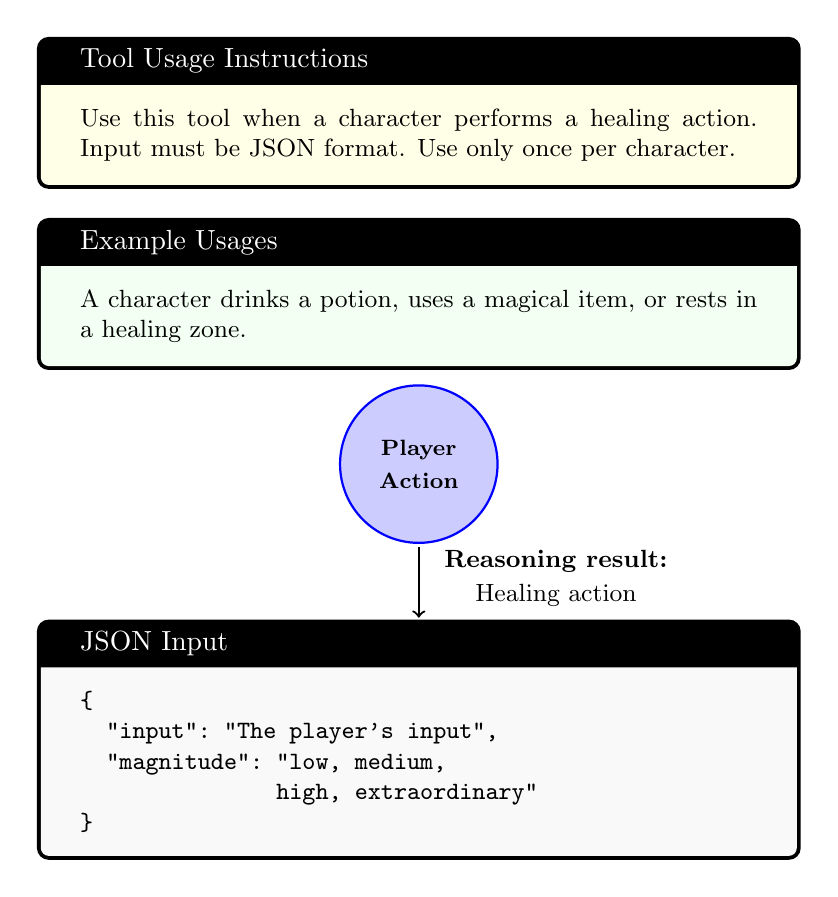
\begin{tikzpicture}
        % Healing action circle
        \draw[fill=blue!20, draw=blue, thick] (0, -1.65) circle (1.0cm);
        \node[text width=1.5cm, align=center] at (0, -1.65) {\footnotesize\textbf{Player Action}};

        % Arrow pointing down
        \draw[->, thick] (0, -2.7) -- (0, -3.6);
        \node[anchor=west, align=center] at (0.2, -3.1) {\small \textbf{Reasoning result:}\\ \small Healing action};

        % JSON Input Box below
        \node[anchor=north] at (0, -3.5) {
 %           \begin{adjustbox}{width=0.3\columnwidth}
            \begin{tcolorbox}[colback=gray!5, colframe=black, title=JSON Input, width=0.8\columnwidth, fontupper=\small]
\begin{verbatim}
{
  "input": "The player's input",
  "magnitude": "low, medium, 
               high, extraordinary"
}
\end{verbatim}
            \end{tcolorbox}
%            \end{adjustbox}
        };

        % Instructions box above
        \node[anchor=north] at (0, 3.9) {
 %           \begin{adjustbox}{width=0.3\columnwidth}
            \begin{tcolorbox}[colback=yellow!10, colframe=black, title=Tool Usage Instructions, width=0.8\columnwidth, fontupper=\small]
            Use this tool when a character performs a healing action. Input must be JSON format. 
            Use only once per character.
            \end{tcolorbox}
%            \end{adjustbox}
        };

        % Example actions box below JSON
        \node[anchor=north] at (0, 1.6) {
 %           \begin{adjustbox}{width=0.3\columnwidth}
            \begin{tcolorbox}[colback=green!5, colframe=black, title=Example Usages
            , width=0.8\columnwidth, fontupper=\small]
            A character drinks a potion, uses a magical item, or rests in a healing zone.
            \end{tcolorbox}
 %           \end{adjustbox}
        };
    \end{tikzpicture}
    \caption{Illustration of the Narrator's reasoning process of using the HealCharacter tool.}
    \Description{An illustration of the Narrator's reasoning process using the HealCharacter tool. Specifically how it is used to determine if a character performs an action that should heal them.}
    \label{fig:healing-tool}
\end{figure}

As agents utilize tool descriptions to guide their reasoning process, all descriptions follow a standardized pattern to ensure consistent behavior:

\begin{enumerate}
    \item \textbf{When to Use:} This step ensures the tool is invoked only under appropriate circumstances, forming the basis of the \textit{Tool Usage Instructions} component of the reasoning process.
    \item \textbf{Examples of Usage:} This step provides sample scenarios for tool application, directly corresponding to the \textit{Example Usages} component. It enables the Narrator agent to associate specific actions with the respective tool.
    \item \textbf{Input Format:} This step defines the input format, which is crucial for accurate parsing by the tools. All input formats are specified in JSON to support consistent interpretation.
    \item \textbf{Number of Uses in Each Trajectory:} This step determines the permissible frequency of tool use within each ReAct trajectory, which corresponds to a single message from the player. It is vital for ensuring agents adhere to the intended usage limits, incorporated into the \textit{Tool Usage Instructions} component.
\end{enumerate}

By adhering to this structured format, the agents are equipped to make informed, consistent decisions, ensuring the execution of tools within the AI GM framework.


%Benefits of v2 approach compared to v1
%\subsection{Design Innovations}

%ChatRPG v2 introduces a dual-agent system—Narrator and Archivist—that leverages the ReAct framework and memory to simulate human-like GM decision-making. The Narrator dynamically adapts the storyline to player interactions, while the Archivist ensures narrative continuity by managing key game elements. This modular design not only enables richer, emergent gameplay and more natural NPC interactions but also simplifies feature integration. Unlike v1’s monolithic approach, v2 supports seamless upgrades by adding new tools without disrupting existing functionality.

\section{Experimental Protocol}
\label{sec:evaluation}
\subsection{Model and Dataset}
\begin{figure}[t]
    \centering
\includegraphics[width=\linewidth]{fig/instruction.png}
    \caption{Instructions given to the LLM for the bias detecrtion.}
    \label{fig:instruction}
\end{figure}
We utilized Stable Diffusion 3.5-large~\cite{sd3} as our text-to-image (T2I) model and employed GPT-4o~\cite{gpt4} for bias detection as a blackbox model, and DeepSeek-V3~\cite{liu2024deepseek} as an open-sourced model. The LLM receives prompts as illustrated in Figure \ref{fig:instruction}. Through in-context learning techniques, we enhance model performance by exposing it to an exemplar task~\cite{brown2020language}. To evaluate the debiasing performance for occupations, we used the occupation dataset from Stable Bias~\cite{Luccioni_2023} (hereafter referred to as the stable bias profession dataset), which contains 131 occupations sourced from the U.S. Bureau of Labor Statistics (BLS). The dataset composition is detailed in the Appendix A of~\cite{Luccioni_2023}. All input prompts were formatted as ``A portrait photo of [profession]'' to ensure that the T2I model interprets them specifically as occupations rather than other potential meanings. To assess the performance in removing implicit social biases present in prompts beyond occupations, we used the Parti Prompt dataset~\cite{yu2022scaling}, which consists of over 1,600 diverse English prompts designed to comprehensively evaluate text-to-image generation models and test their limitations. For attribute rebalancing, we employed the uniform distribution, as our primary goal was to verify the debiasing capability of our latent variable guidance.

% For experiments involving bias adjustment using employment statistics log-probabilities, we conducted experiments to mitigate gender bias using BLS2022 statistical data for five occupation prompts mentioned in \cite{naik2023social}: ``CEO'', ``doctor'', ``computer programmer'', ``house keeper'', and ``nurse''.

\subsection{Human Evaluation}
For each prompt, nine images are generated using three methods: a baseline method without debiasing, and two LLM-assisted debiasing methods employing GPT-4o and DeepSeek-V3. These images are arranged in a 3 $\times$ 3 grid, and evaluators assess pairs of images based on image quality, prompt reflection, and diversity of generations. Image quality refers to the aesthetic appeal, high resolution, natural appearance, and detailed refinement of the images. Prompt adherence measures the degree to which the generated images reflect the input text. Diversity of generations evaluates the variety of generated results, particularly whether the images avoid stereotypes and fixed patterns. For each criterion, evaluators rate the results on a 5-point scale, ranging from 1 (very poor) to 5 (very good). To facilitate relative comparisons, images generated by different models for the same input prompt are presented in consecutive questions. This comparative evaluation across the three criteria enables a detailed assessment of the proposed methods' relative strengths and limitations. We randomly selected 50 prompts from Stable Bias profession dataset and Parti Prompt dataset. The subset used for the human evaluation is detailed in Table\ref{tab:sd_subset} and Table\ref{tab:pp_subset} in the supplementary materials. Responses were collected from 20 evaluators, ensuring a diverse range of perspectives. 
\subsection{Non-parametric Evaluation}
Quantitative evaluation of generation diversity presents significant challenges. To address this, we adopt the clustering-based evaluation methodology proposed in Stable Bias~\cite{Luccioni_2023}, implementing a nonparametric diversity assessment using k-Nearest Neighbors (kNN)~\cite{fix1985discriminatory}. Specifically, we generate anchor images based on prompts structured as ``a portrait of a [ethnicity] [gender] at work,'' creating nine images for each combination of ethnicity and gender. This analysis employs 18 ethnic labels from Stable Bias and three gender categories: ``male'', ``female'', and ``non-binary'' (detailed ethnic labels are provided in the Appendix A of~\cite{Luccioni_2023}).

For image embeddings, we utilize Google's VertexAI multimodal embedding model\footnote{https://cloud.google.com/vertex-ai/docs/generative-ai/embeddings/get-multimodal-embeddings}, which converts 512 $\times$ 512 images into 1048-dimensional vector representations. For each prompt in the identity dataset, 30 unique images are generated, yielding a total of 54 $\times$ 30 $=$ 1620 images that serve as anchor points for classification. To examine local trends linked to specific professions, we follow the methodology outlined in \cite{naik2023social}, generating 210 images per method for five professions: ``CEO'', ``computer programmer'', ``doctor'', ``nurse'', and ``housekeeper''. The classification results are visualized to uncover potential biases or distinct patterns specific to each profession.

% In addition, to capture global trends across the entire profession dataset, we generate nine images per profession prompt for each method. These classification results provide an overarching perspective on diversity and potential biases in the generated outputs.


\section{Discussion}
\label{sec:discussion}

% \TODO{Bryan}

Our multimodal data augmentation method is a plug-and-play method that can be applied to any future VLM. Also the T2I generation can be replaced by any future T2I model, thus the effectiveness of our method automatically improves along with the SOTA T2I model, making it future-proof.



Our main method, \textbf{Co}ntrastive Visual \textbf{D}ata \textbf{A}ugmentation (\textbf{CoDA}), is simple and easy to apply to LMMs in a variety of scenarios. Several components in the pipeline utilize existing off-the-shelf model components that can be easily swapped out for superior versions of similar models as research in their respective field progresses. Therefore, we expect the efficiency and effectiveness of \textbf{CoDA} to dramatically scale along with the advancement of relevant models. 



\section{Conclusion and future directions} \label{sec:conclusion}

In this paper we proposed a nested MLMC framework that offers important computational savings by performing most calculations in low precision and exploiting approximate random normal variables for the low precision path calculations. The low precision calculations could be performed in fixed precision on an FPGA for greater efficiency, and we suggested a procedure to optimise the bit-widths of every variable at each Monte Carlo level. This is an important improvement over previous mixed precision MLMC frameworks which held the lower precision fixed \cite{Rounding_error_oliver} or defined uniform bit-width at every level heuristically \cite{brugger2014mixed}. Our numerical results suggest that for the first levels our procedure reduces the cost at these levels by a factor 5 or 7. Hence the overall savings are significant since most paths are calculated on the first levels. Our approach would be even more efficient for the Milstein scheme because its higher order strong convergence leads to a greater proportion of the computational costs being on the coarsest levels.

The next stage of the research project will be to implement the RNG methods and the nested framework on FPGAs to determine the hardware requirements and confirm the extent of the computational savings. It would also be good to compare the performance benefits to using half-precision floating point arithmetic on GPUs or CPUs for the low-accuracy computations.





%%
%% The acknowledgments section is defined using the "acks" environment
%% (and NOT an unnumbered section). This ensures the proper
%% identification of the section in the article metadata, and the
%% consistent spelling of the heading.

\begin{acks}
We sincerely thank the 12 test participants whose contributions through user tests were essential in shaping the outcomes of this study.
\end{acks}

%%
%% The next two lines define the bibliography style to be used, and
%% the bibliography file.
\bibliographystyle{ACM-Reference-Format}
\balance
\bibliography{references}


%%
%% If your work has an appendix, this is the place to put it.
\appendix



\include{0_appendiks/1_appendiks}


%%\section{Research Methods}

\end{document}
\endinput
%%
%% End of file `sample-sigconf-authordraft.tex'.
